%%%%%%%%%%%%%%%%%%%%%%%%%%%%%%%%%%%%%%%%%%%%%%%%%%%%%%%%%%%%%%%%%%%%%%%%
%    INSTITUTE OF PHYSICS PUBLISHING                                   %
%                                                                      %
%   `Preparing an article for publication in an Institute of Physics   %
%    Publishing journal using LaTeX'                                   %
%                                                                      %
%    LaTeX source code `ioplau2e.tex' used to generate `author         %
%    guidelines', the documentation explaining and demonstrating use   %
%    of the Institute of Physics Publishing LaTeX preprint files       %
%    `iopart.cls, iopart12.clo and iopart10.clo'.                      %
%                                                                      %
%    `ioplau2e.tex' itself uses LaTeX with `iopart.cls'                %
%                                                                      %
%%%%%%%%%%%%%%%%%%%%%%%%%%%%%%%%%%
%
%
% First we have a character check
%
% ! exclamation mark    " double quote  
% # hash                ` opening quote (grave)
% & ampersand           ' closing quote (acute)
% $ dollar              % percent       
% ( open parenthesis    ) close paren.  
% - hyphen              = equals sign
% | vertical bar        ~ tilde         
% @ at sign             _ underscore
% { open curly brace    } close curly   
% [ open square         ] close square bracket
% + plus sign           ; semi-colon    
% * asterisk            : colon
% < open angle bracket  > close angle   
% , comma               . full stop
% ? question mark       / forward slash 
% \ backslash           ^ circumflex
%
% ABCDEFGHIJKLMNOPQRSTUVWXYZ 
% abcdefghijklmnopqrstuvwxyz 
% 1234567890
%
%%%%%%%%%%%%%%%%%%%%%%%%%%%%%%%%%%%%%%%%%%%%%%%%%%%%%%%%%%%%%%%%%%%
%
\documentclass[12pt]{iopart}
\usepackage {latexsym}
\usepackage {graphicx}
\usepackage{iopams}
\usepackage {color}

%\documentclass[12pt]{iopart}
%\newcommand{\gguide}{{\it Preparing graphics for IOP journals}}
%Uncomment next line if AMS fonts required
%\usepackage{iopams}  
%\usepackage {amsmath}
%\usepackage {amssymb}
%\usepackage {amsfonts}
%\usepackage {amsthm}
%\usepackage {mathrsfs}
%\usepackage {natbib}
%\usepackage {latexsym}
%\usepackage {graphicx}
%\usepackage {dsfont}
%\usepackage {times}
%\usepackage {txfonts}
%\usepackage {rotating}
%\usepackage {wasysym}
%\usepackage {multirow}
%\usepackage {hhline}
\usepackage {hyperref}
%\usepackage {color}
\usepackage {bm}
%\usepackage{appendix}
\usepackage{acronym}
%\usepackage{dcolumn}   % needed for some tables
\usepackage {url}
%\usepackage[normalem]{ulem}   % temporal one in draft.

% variable shortcuts 
\newcommand{\Hub}{H_{0}}
\newcommand{\DL}{D_{\mathrm{L}}}
\newcommand{\lam}{\bm{\lambda}}
%\newcommand{\data}{\bm{d}}
%\newcommand{\sigpar}{\bm{\theta}}
%\newcommand{\nuispar}{\bm{\lambda}}
%\newcommand{\globpar}{\bm{\gamma}}
%\newcommand{\model}{\mathcal{H}}

\newcommand{\curlH}{\mathcal{H}}
\newcommand{\gws}{\tilde{h}}

%% ----- input git-version tag
\input{tag.tex}

\newcommand{\dcc}{LIGO-PXXXXXXXX}
\newcommand{\cm}[1]{\textcolor{red}{CM: #1}}
\newcommand{\MP}[1]{\textcolor{blue}{MP: #1}}
\newcommand{\lw}[1]{\textcolor{green}{LW: #1}}

\newcommand{\aap}{A\&A }
\newcommand{\apj}{ApJ  }
\newcommand{\apjl}{ApJL  }
\newcommand{\apjs}{ApJS  }
\newcommand{\prd}{Phys. Rev. D  }
\newcommand{\nat}{Nature}
\newcommand{\araa}{ARA\&A}
\newcommand{\mnras}{Monthly Notices of the Royal Astronomical Society  }
\begin{document}

\title{Astrophysical calibration of gravitational-wave detectors}

\author{L.~Wright$^1$, M.~Pitkin$^1$ \& C.~Messenger$^1$}
\address{$^1$ SUPA, School of Physics and Astronomy, University of
  Glasgow, Glasgow G12 8QQ, United Kingdom}
\ead{1002990W@student.gla.ac.uk}

\begin{abstract}
  We present an investigation into the potential of calibrating \MP{change to: ``assessing the validity of the calibration''?}
  gravitational wave detector outputs through the use of standard
  sirens. Such signals, as measured via gravitational wave
  observations provide an estimated luminosity distance which is
  subject to uncertainties in the calibration of the data.  If a host
  galaxy is identified for a given source then its redshift can be
  obtained and combined with current knowledge of the cosmologic
  parameters.  This will yield the true luminosity distance and allow
  the direct comparison with the estimated value.  Discrepancies can
  then be used to correct the original calibration.~\cm{Update at end}
\end{abstract}

% acronym definitions
\acrodef{GW}[GW]{gravitational wave}
\acrodef{BNS}[BNS]{binary neutron star}
\acrodef{MWEG}[MWEG]{Milky Way equivelent galaxies}
\acrodef{BBH}[BBH]{binary black hole}
\acrodef{NSBH}[NSBH]{neutron star black hole}
\acrodef{SNR}[SNR]{signal-to-noise ratio}
\acrodef{GRB}[GRB]{gamma-ray burst}
\acrodef{sGRB}[sGRB]{short gamma-ray burst}
\acrodef{CBC}[CBC]{compact binary coalescence}
\acrodef{EM}[EM]{electro-magnetic}

%Uncomment for PACS numbers title message
%\pacs{00.00, 20.00, 42.10}
% Keywords required only for MST, PB, PMB, PM, JOA, JOB? 
%\vspace{2pc}
%\noindent{\it Keywords}: Article preparation, IOP journals
% Uncomment for Submitted to journal title message
%\submitto{\JPA}
% Comment out if separate title page not required
\maketitle

%%%%%%%%%%%%%%%%%%%%%%%%%%%%%%%%%%%%%%%%%%%%%%%%%%
%%%%%%%%%%%%%%%%%%%%%%%%%%%%%%%%%%%%%%%%%%%%%%%%%%
\section{Introduction\label{sec:intro}}

% introduce GWs and BNS systems
It is expected that the advanced generation of interferometric \ac{GW}
detectors will detect waves emitted from $O(10s)$ of compact binary
coalescences.  One such class of these cataclysmic events, the inspiral and
merger of \ac{BNS} systems will be detected out to a maximum range of $\approx
450$ Mpc. Assuming the current best estimates for the cosmological parameters,
this is equivelent to a redshift $z\approx 0.1$. As noted by~\cite{} \ac{CBC}
systems can be used as cosmiological distance markers, otherwise known as
``standard sirens'' (analogous to the \ac{EM} standard candles). Standard sirens
allow ...

% BNS systems are GRBs
It is considered likely that the merger of \ac{BNS} systems, in addition to
emitting detectable \acp{GW}, is also the mechanism for producing \acp{sGRB}.
In this scenario these \ac{EM} events are produced through the ... and result
in tightly beamed emission parallel to the orbital angular momentum vector of
the \ac{BNS} system. Additional evidence for the coincidence of \acp{sGRB} with
\ac{GW} events are the estimated astrophysical rates of both phenomena.
Observations of \acp{sGRB} give a rate of XXX Mpc$^{-3}$yr$^{-1}$ which can be
compared to estimates of \ac{BNS} merger rates of XXX-XXX Mpc$^{-3}$yr$^{-1}$.
This latter range is obtained from population synthesis models together with
knowledge of the X known \ac{BNS} systems in our galaxy. 
  
% talk about the calibration idea
If a single \ac{GW} event is observed in coincidence with a \ac{sGRB} it will \MP{may?}
be possible to identify the host galaxy of the \ac{BNS} source.  With this
information a spectroscopic redshift can be very accurately obtained. With
knowledge of the redshift, using current best estimates for the Hubble constant
and other cosmological parameters, the true luminosity distance can be
estimated to $\sim 1\%$ accuracy.  The \ac{GW} measurement acts as a standard
siren also giving us a direct measurement of the luminosity distance to the source.
The accuracy of such a measurement depends on a number of factors including the
accuracy with which the \ac{GW} detector has been calibrated.  Hence comparison
with the distance estimate from the \ac{sGRB} we can re-calibrate (or validate)
the existing experimentally obtained calibration. 

% What do we do in this paper
In this paper we investigate the feasibility of this approach for single
coincident \ac{GW}--\ac{sGRB} events and establish the validation power of such
a calibration technique.  In Sec.~\ref{sec:calibration} we briefly summarize
the existing experimental technique for \ac{GW} detector calibration and its
expected accuracy.  We then review the concept of \ac{GW} standard sirens and
their proposed coincident \ac{EM} signatures, the \acp{sGRB} in
Secs.~\ref{sec:sirens} and~\ref{sec:GRB}. In Sec.~\ref{sec:single} we present
the results of Monte-Carlo simulations for the purpose of luminosity distance
estimation using \ac{GW} events. In Sec.~\ref{sec:cosmo} we show the likely
accuracy of \ac{sGRB} distances obtained from their host galaxy redshift and in
Sec.~\ref{sec:discussion} we conclude.    

%%%%%%%%%%%%%%%%%%%%%%%%%%%%%%%%%%%%%%%%%%%%%%%%%%
%%%%%%%%%%%%%%%%%%%%%%%%%%%%%%%%%%%%%%%%%%%%%%%%%%
\section{Gravitational wave detector calibration\label{sec:calibration}}

\cm{We need to define our model for the calibration, i.e. are we talking
about amplitude only and are we breaking this up over frequency.}

\MP{In this paper I think we stick to just talking about a single overall amplitude calibration scale.}

The technique used throughout GW research in calibrating the detectors is
carried out through a complicated system of physical manipulations of the
Fabret-Perot Michelson interferometer; where an elaborate feedback system is
used to sustain a defined measurement in arm length difference between the
moving mirrors~\cite{LIGOCal}. In general, the interferometers are set to move
at a frequency corresponding to a GW signal. An error signal is then found
through the Pound-Driver-Hall technique~\cite{Black} for mirror stabilisation
which is proportional to the difference in mirror separation of the
Fabret-Perot Michelson interferometer. The Pound-Drever-Hall technique is
essentially a control loop feedback system in which the difference output (in
GW detectors, this is the distance the mirrors move due to the GW) and the the
output set is reduced to the highest degree of certainty. This is just a brief
overview of the calibration method currently used, and is an extensive study in
itself, see~\cite{Vitale:2012} and references therein. For advanced LIGO and Virgo,
at the frequency range used in this project, the error in the calibration using
the `hardware injection method' is roughly $10\%$~\cite{Vitale:2012}. This is a
benchmark set for the error estimation using the proposed new method in this
project.~\cm{Clean this up and expand.}

% Describe our model for the calibration
In this work the calibration correction factor used throughout is simply a scale
factor, $s$. This effects the data set collected by a simple multiplication:
%
\begin{equation}\label{eq:scaledata}
  h(t) = s\times h_{\mathrm{m}}(t)
\end{equation}
%
where $h_{\mathrm{m}}(t)$ is the measured detector strain, and
$h(t)$ is the exact perfectly calibrated strain. A description of the
collected data is given in Section~\ref{sec:cbc}. The scale factor being
parameterised, $s$, represents all known sources of error in the system. This
is not entirely realistic as $s$ is known to be a function of frequency.
Testing a more realistic calibration error is work to be done in the
future.~\cm{Need to clean this up and expand the discussion}

%%%%%%%%%%%%%%%%%%%%%%%%%%%%%%%%%%%%%%%%%%%%%%%%%%
%%%%%%%%%%%%%%%%%%%%%%%%%%%%%%%%%%%%%%%%%%%%%%%%%%
\section{Binary neutron star standard sirens\label{sec:sirens}}

We should explain what this means starting with reference
to~\cite{1986Natur.323..310S}.

%%%%%%%%%%%%%%%%%%%%%%%%%%%%%%%%%%%%%%%%%%%%%%%%%%
%%%%%%%%%%%%%%%%%%%%%%%%%%%%%%%%%%%%%%%%%%%%%%%%%%
\section{GRB counterparts\label{sec:GRB}}

% what are sGRBs 
\cm{What are sGRBs?}\\

% discuss joint-event rates
\cm{Discuss the expected rate of joint detections}\\

% observing a coincident event
The most likely scenario in which a coincident \ac{GW}--\ac{sGRB} event would
be identified is through the targeted follow-up of an observed \ac{sGRB} or by
post-facto matching of \ac{GW} trigger lists with known \ac{sGRB} events.  The
likelihood of being able to follow-up \ac{GW} events using gamma-ray telescopes
with low enough latency to catch a \ac{sGRB} is low.  Compounding this issue is
the relatively large \ac{GW} sky error-box giving a field-of-view for the
\ac{EM} observatories to search spanning $\sim 100$'s of square
degrees~\cite{grb}.  For the \ac{GW} follow-up of \ac{sGRB} scenario the merger
time for \ac{BNS} systems will be estimated from the \ac{sGRB} to within a few
seconds~\cite{grb}.  This makes the follow-up search less computationally
expensive since it is performed over a smaller range of data using potentially
fewer numbers of waveform templates.  This computational saving enables the use
of a more computationally expensive multi-detector coherent scheme rather than
the cheaper coincidence methods used in the untargeted searches. 

% discuss the inclination angle issue
A fortunate consequence of a joint \ac{GW}--\ac{sGRB} observation will be the
fact that in order for such an event to be observed, the \ac{BNS} system must
have had its orbital angular momentum vector pointing towards (or away) from
the detector.  The actual inclination angle of the system, defined as the angle
between the orbital angular momentum vector and the line of sight, must be $<$
half of the \ac{sGRB} beaming angle.  This prerequisite property limits us to
systems that are approximately ``face-on'' and therefore biases us to higher
\ac{SNR} signals.  However, as discussed earlier, the property of beaming
severely impacts the probable rate of such joint observations.   


%%%%%%%%%%%%%%%%%%%%%%%%%%%%%%%%%%%%%%%%%%%%%%%%%%
%%%%%%%%%%%%%%%%%%%%%%%%%%%%%%%%%%%%%%%%%%%%%%%%%%
\section{A single event with GRB counterpart\label{sec:single}}

\cm{This should be the simplest case we can do.  We need to cut a lot of this.}

% Describe what we are going to do in this section
Let us consider a single \ac{GW} detection of the inspiral stage of a \ac{BNS}
merger and assume that this signal has been associated with a potential
\ac{sGRB} detection. We therefore also assume that the inclination angle
of the binary is consistent with a given \ac{sGRB} beaming angle.  Finally we
assume that a host galaxy has been identified for the source and that the sky
position is therefore known to high precision. 
 
% Describe the signal model (Taylor F2 etc...)
We use the post-Newtonian Taylor F2 waveform approximation for modelling the
signal whereby the \ac{GW} phase for 2 point-particles of mass $m_{1}$ and
$m_{2}$ is given by
%
\begin{equation}
\label{eq:gwphase}
  \Psi(f) = 2\pi f t_\mathrm{c} - \phi_{\mathrm{c}} - \frac{\pi}{4} +
\frac{3}{128\eta\nu^{5}}\sum\limits_{k=0}^{7}\alpha_{k}\nu^{k}.
\end{equation}
%
Here $\eta=m_{1}m_{2}/M^{2}$ is the symmetric mass-ratio with $M=m_{1}+m_{2}$
the total mass.  The post-Newtonian expansion parameter is $\nu=(\pi M
f)^{1/3}$ and the coefficients are $\alpha$.

The frequency-domain polarisation amplitudes are then defined as
%
\begin{eqnarray}
  \gws_{+}(f) &=& \frac{1+\cos^{2}\iota}{2D_{L}}
\frac{\mathcal{M}^{5/6}}{\pi^{2/3}}
\sqrt{\frac{5}{24}}f^{-7/6}e^{-i\Psi(f)}\\
  \gws_{\times}(f) &=&
 i\frac{\cos^{2}\iota}{D_{L}}\frac{\mathcal{M}^{5/6}}{\pi^{2/3}}
\sqrt{\frac{5}{24}}f^{-7/6}e^{-i\Psi(f)}
\end{eqnarray}
%
where the chirp-mass $\mathcal{M}$ is defined as $\mathcal{M}=M\eta^{3/5}$,
and $\iota$ is the inclination angle.  The \ac{GW} strain measured
at the $k$'th detector is then given by
%
\begin{equation}
  \label{eq:gravsig}
   \gws^{k}(f) = \big[ F_{+}^{k}(\alpha, \delta, \psi)\gws_{+}(f) +
F_{\times}^D(\alpha, \delta, \psi)\gws_{\times}(f)\big]
\end{equation}
%
where $F_{+},F_{\times}$ are the antenna response functions which are dependent
upon the polarisation angle $\psi$ and the sky position of the source
$\alpha,\delta$.

% Define the detectors and the noise epoch we will be using
For this analysis we will consider advanced generation instruments operating
at their design sensitivity.  The network we consider is the 3 detector
H1--L1--V1 configuration. 

% Define the likelihood function we will be using
We consider that the measured data in any detector is defined as
%
\begin{equation}
  d^{k}(f)=\tilde{n}^{k}(f)+s\gws_{k}(f)
\end{equation}
%
where $\tilde{n}(f)$ is the Fourier transform of Gaussian noise drawn from a
distribution consistent with the power-spectral-density of the advanced
detector noise.  The likelihood function for application to discretely sampled
data is 
%
\begin{equation}
  p(\vec{d} | \vec{\theta}, \curlH, I) \propto \exp\Bigg[ 2\Delta
f\sum_{k>0}\frac{|\tilde{d}(f_{k}) - \tilde{h}(f_{k})|^{2}}{S(f_{k})}\Bigg]
\end{equation}
% 
where $\Delta f$ is the frequency resolution of the frequency domain data. 

% describe what parameters we will be considering and their priors
We assume uniform prior distributions on the unknown nuisance parameters
$\phi_{\mathrm{c}},\psi$ on their standard ranges. The time of coalescence is
restricted to a prior range of $\pm 10$ msec around the true value.  Given our
assumption of an \ac{sGRB} counterpart and host galaxy, we treat the sky
position as exactly known. We also consider the cosine of the inclination angle to be drawn
from a zero-mean Gaussian with standard deviation $0.1$ consistent with an
uncertainty on \ac{sGRB} opening of XXX~\cm{What was exactly done here?}.  The
main parameter of interest, the calibration scale factor $s$ is assumed to have
a uniform prior distribution on the range $(0,2)$.    

% mention the no-noise issue
We note that the analysis performed here used zero-noise realisations in which
no actual noise was added to our signals.  The likelihood functions still
contain the correct \ac{PSD} and hence the accuracy with which the parameters
are recovered (indicated by the widths of the posterior distributions) is
representative of the statistical errors in realistic noise scenarios.

% Describe the ensemble of simulations used




where the noise spectral density, $S^D(f)$ is not a function of distance, shown
in section~\ref{sec:pandl}. For coalescing binary neutron stars of masses
$m_{1,2} = 1.4\,M_{\odot}$ and  $D_{L}200\,Mpc$, the expected SNR is roughly 8.
The SNR was determined from $D_{L} = [10,200]\,Mpc$  using a randomly chosen
sky position which defines the antenna patterns and the GW signal. The range of
luminosity distance used in this paper represented a high level of SNR up to
the distance at which the first predicted detectable GW source; $D_{L} =
200\,Mpc$. The detector limits for the advanced era is a luminosity distance of
$\sim 450\,Mpc$. This was not initially tested as the SNR was low enough to
cause problems with computational time. It was however tested in the random sky
position simulations, see section~\ref{sec:rndsp}. The initial value for the
calibration error used in the analysis was chosen randomly.

\begin{figure}
  \centering
  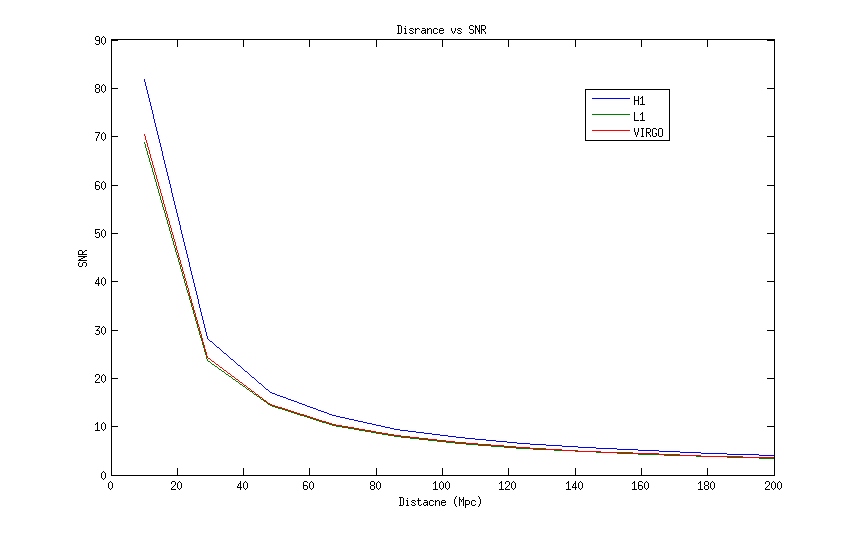
\includegraphics[width = \textwidth]{DvsSNR-mult-det}
  \caption{The distance and SNR relationship for all three detectors:
LIGO Hanford, H1, LIGO Livingston, L1, and VIRGO.}
  \label{fig:distsnr}
\end{figure}

To begin with, parameter estimation was carried out on the simplest case: a
single source of GWs using a single detector, LIGO Hanford, at different levels
of SNR. The aim was to resolve the calibration scale factor with the highest
degree of certainty.  Before testing the uncertainty resolution using a the
full range of prior parameters, we fixed all values to known signal values and
only searched over the scale factor. Results shown for with and without a full
prior range are given in figures~\ref{fig:sd-empty-D}
and~\ref{fig:sd-non-empty-D} respectively.


\begin{figure}
  \centering
  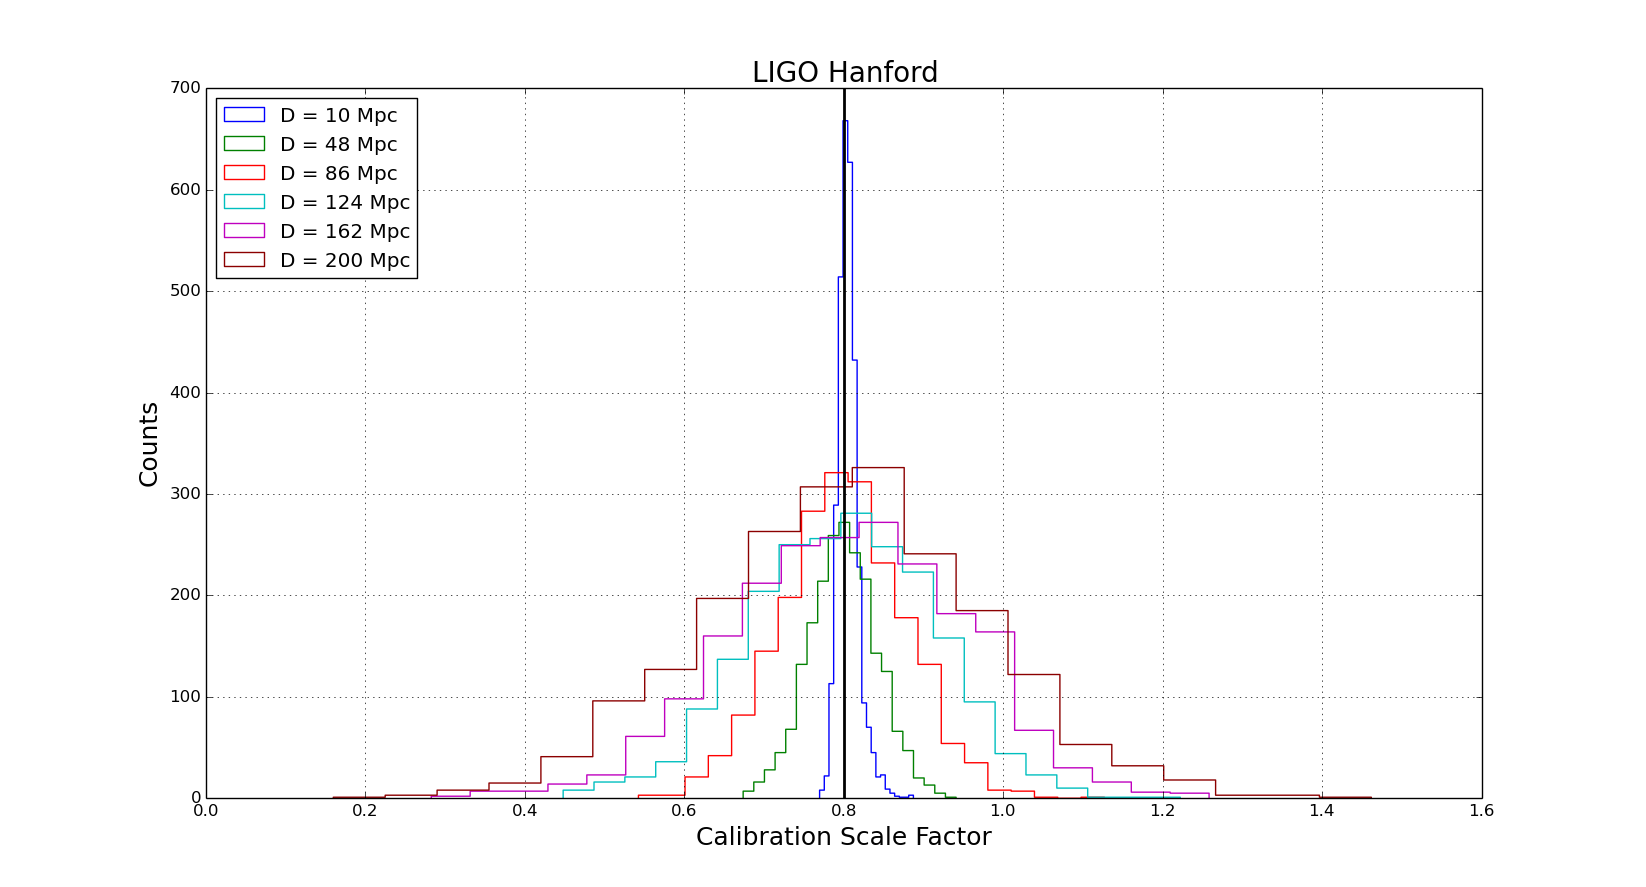
\includegraphics[width = \textwidth]{SD_empty_D10_200}
  \caption{\textit{Posterior distribution on the calibration scale factor for
LIGO Hanford. Simulations carried out using an entirely known source of GWs.}}
  \label{fig:sd-empty-D}
\end{figure}

The figure above is a histogram of the calibration error, with each curve
representing a different distance (SNR). The black line at $s = 0.8$ is the
initial scale factor value used to multiply the unanalysed data set. This
representation of the initial calibration scale factor will be continuous
throughout the paper.  One would expect with lower SNR (greater $D_{L}$), the
estimation of the parameter would become less certain. This is clearly shown in
figure~\ref{fig:sd-empty-D} as the standard deviations of the curves increases
with smaller SNR/larger luminosity distances. For this entirely known source of
GWs, we would expect to find the uncertainty in $s$ to be approximately
$1/$SNR; this is what we see in figure~\ref{fig:sd-empty-D}. The error in
estimating $s$ for $D_{L} = 200 \,Mpc$ is roughly $\sim 20\%$. This is larger
than the current method of obtaining the uncertainty in calibration. A full
test of the new method proposed is carried out in section~\ref{sec:rndsp}.

The next estimation of the calibration scale factor was performed with a full
range of prior parameters, giving a more realistic system. As before, the
simulations were carried out for differing levels of SNR and a histogram of the
calibration error was made, seen in figure~\ref{fig:sd-non-empty-D}.

\begin{figure}
  \centering
  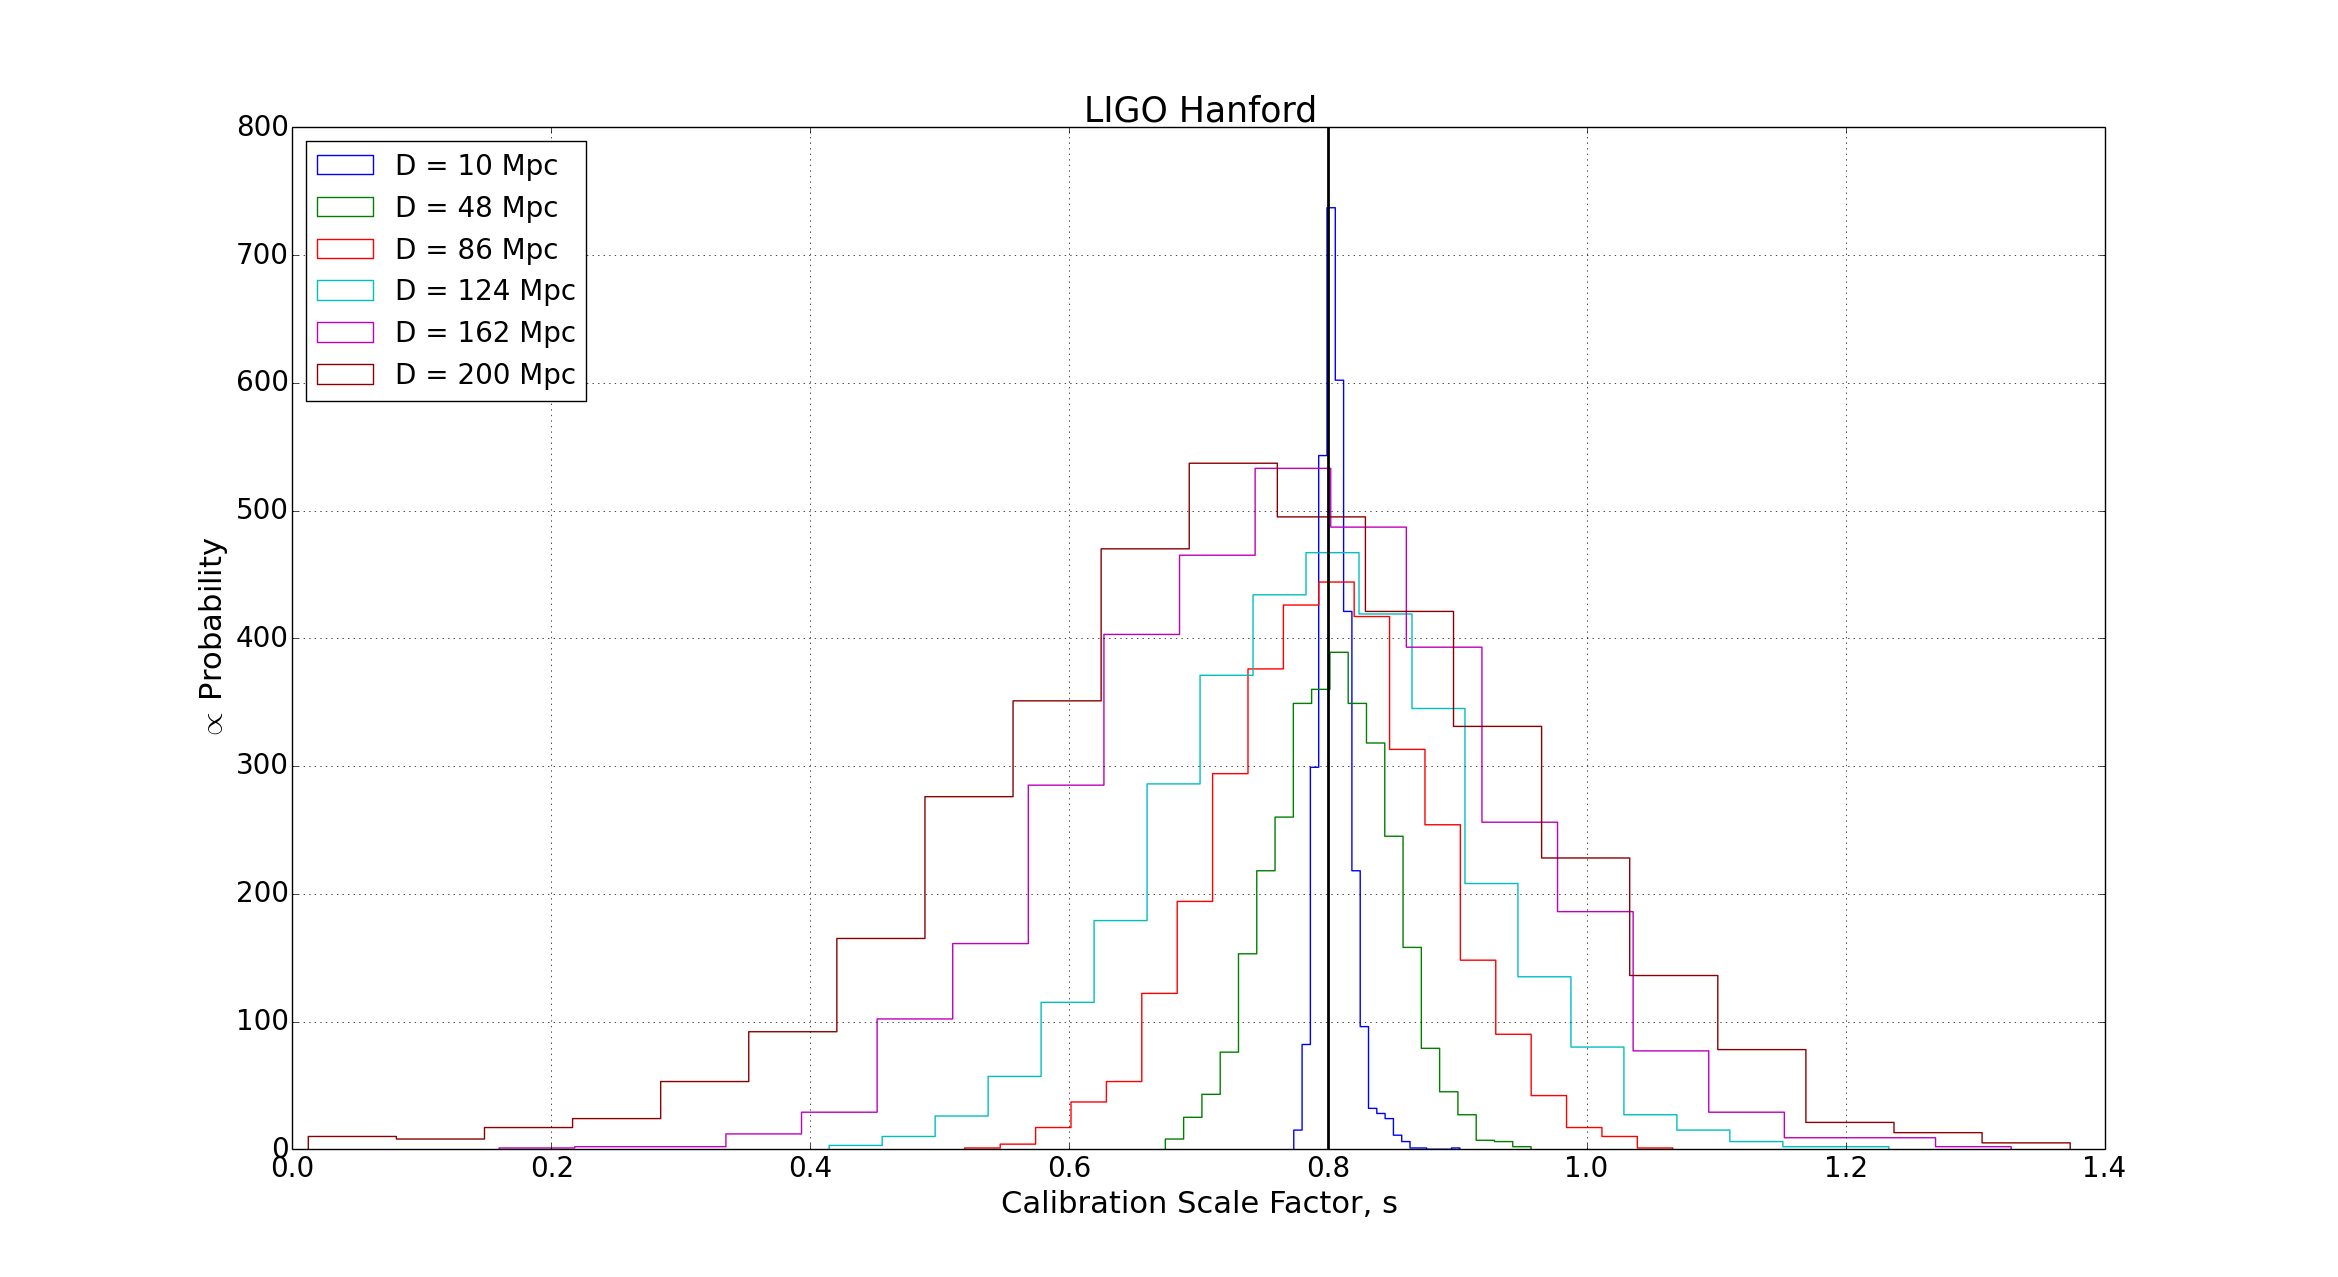
\includegraphics[width = \textwidth]{SD_non_empty_D10_200}
  \caption{\textit{Posterior distribution on the calibration scale factor for
LIGO Hanford. Simulations carried out with some parameters in the prior.}}
  \label{fig:sd-non-empty-D}
\end{figure}

The error in the calibration scale factor, as before, increases with decreasing
SNR (increasing $D_{L}$). The magnitude of this error however is larger than in
the previous simulation. With a full prior range given in
section~\ref{sec:pandl}, the standard deviation increases; at $D_{L} =
200\,Mpc$ the error in $s$ is $\sim 24\%$. When comparing this new method of
calibration scale factor estimation with the current, feedback loop system
method used today, this method is not as accurate. However, it should again be
noted that this method is an independent estimate of the calibration accuracy.

A network of detectors are used throughout GW research. Being able to show the
effect of the calibration error and recovering its uncertainty in the analysis
would help in giving a detection more confidence. In this section, the
simulations were carried out using multiple detectors; LIGO Hanford, LIGO
Livingston, and Virgo. In reality, multiple detectors are used in order to
determine the (rough) sky position of a signal. Due to their locations, if one
site detects a signal before the others, then the position of the source can be
roughly worked out. The aim was, as before, to estimate the calibration scale
factor with the least amount of uncertainty for differing levels of SNR for a
single source of GWs.

For a network of detectors, the overall likelihood function becomes a product
of each likelihood for all detectors, i.e.

\begin{equation}
  \label{eq:mult-likeli}
  p(\vec{d}| \vec{\theta}, \curlH) = \prod \limits_D p(\vec{d}^D| \vec{\theta},
\curlH)
\end{equation}

where $D = \{H,L,V\}$. The initial calibration scale factors where again chosen
at random ($s = [4.6, 2.5, 6.1]$ for LIGO Hanford, LIGO Livingston, and Virgo
respectively). The simulations were the same as before, using the same
parameter values. The GRB assumption was again tested in these simulations as a
handful of parameters were relaxed and given some uncertainty. The results of
these simulations are shown in figure~\ref{fig:mult-empty-D} and
figure~\ref{fig:mult-non-D}.

\begin{figure}
  \centering
  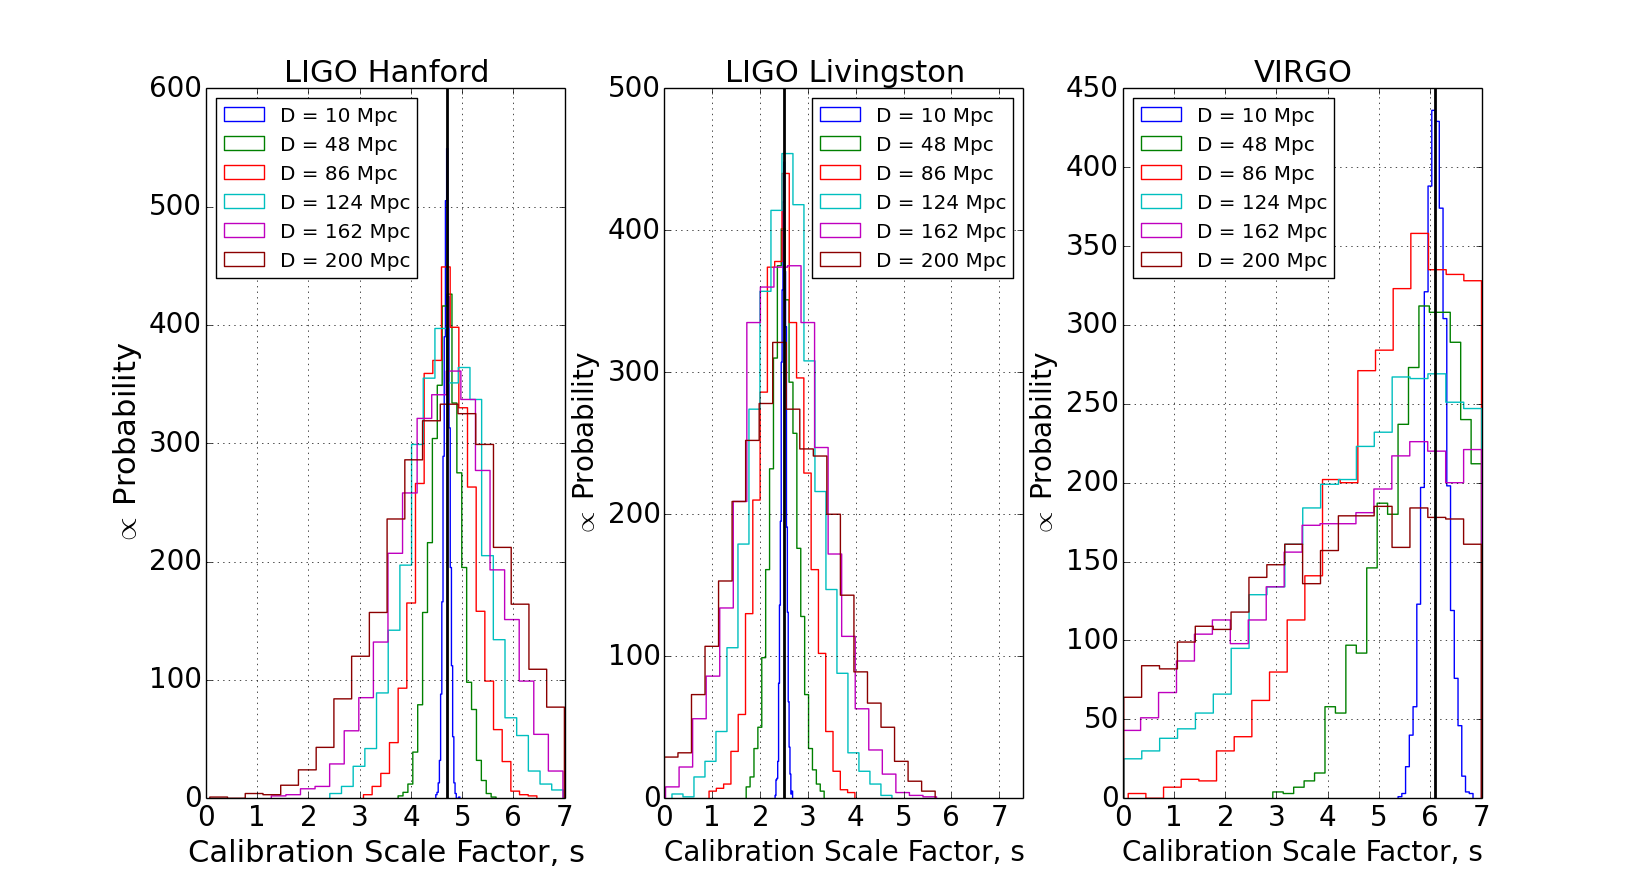
\includegraphics[width = \textwidth]{MD_empty_D10_200}
  \caption{Posterior distribution on the calibration scale factor for
all three detectors. Simulations carried out using an entirely known source of
GWs.}
    \label{fig:mult-empty-D}
\end{figure}

Figure~\ref{fig:mult-empty-D} shows the histograms of the calibration scale
factor for each detector. These simulations used an entirely known source of
GWs, at a randomly chosen sky position (the same sky position as before). As
the figure shows both LIGO sites, Hanford and Livingston, are able to resolve
the error with a measurable degree of uncertainty. The standard deviation for
$s$ at $D_{L}=200\,Mpc$ is $24\%$ and $41\%$ of the true scale factor for
Hanford and Livingston respectively. The estimation for the calibration error
using VIRGO however, was not as accurate. It can be seen that, for increasing
luminosity distances, the resolution of $s$ becomes increasingly uncertain
until the point at which the distribution becomes almost uniform; $D_{L}
\approx 120\,Mpc$. There are a few reasons why this may be. Firstly, the sky
position used may not be 'ideal' for generating the antenna patterns. The most
probable cause of the estimation being very poor will lie in the detector
itself. The interferometer itself is not as sensitive the two LIGO sites, hence
the estimation of parameters using this site will not be as precise.

\begin{figure}
  \centering
  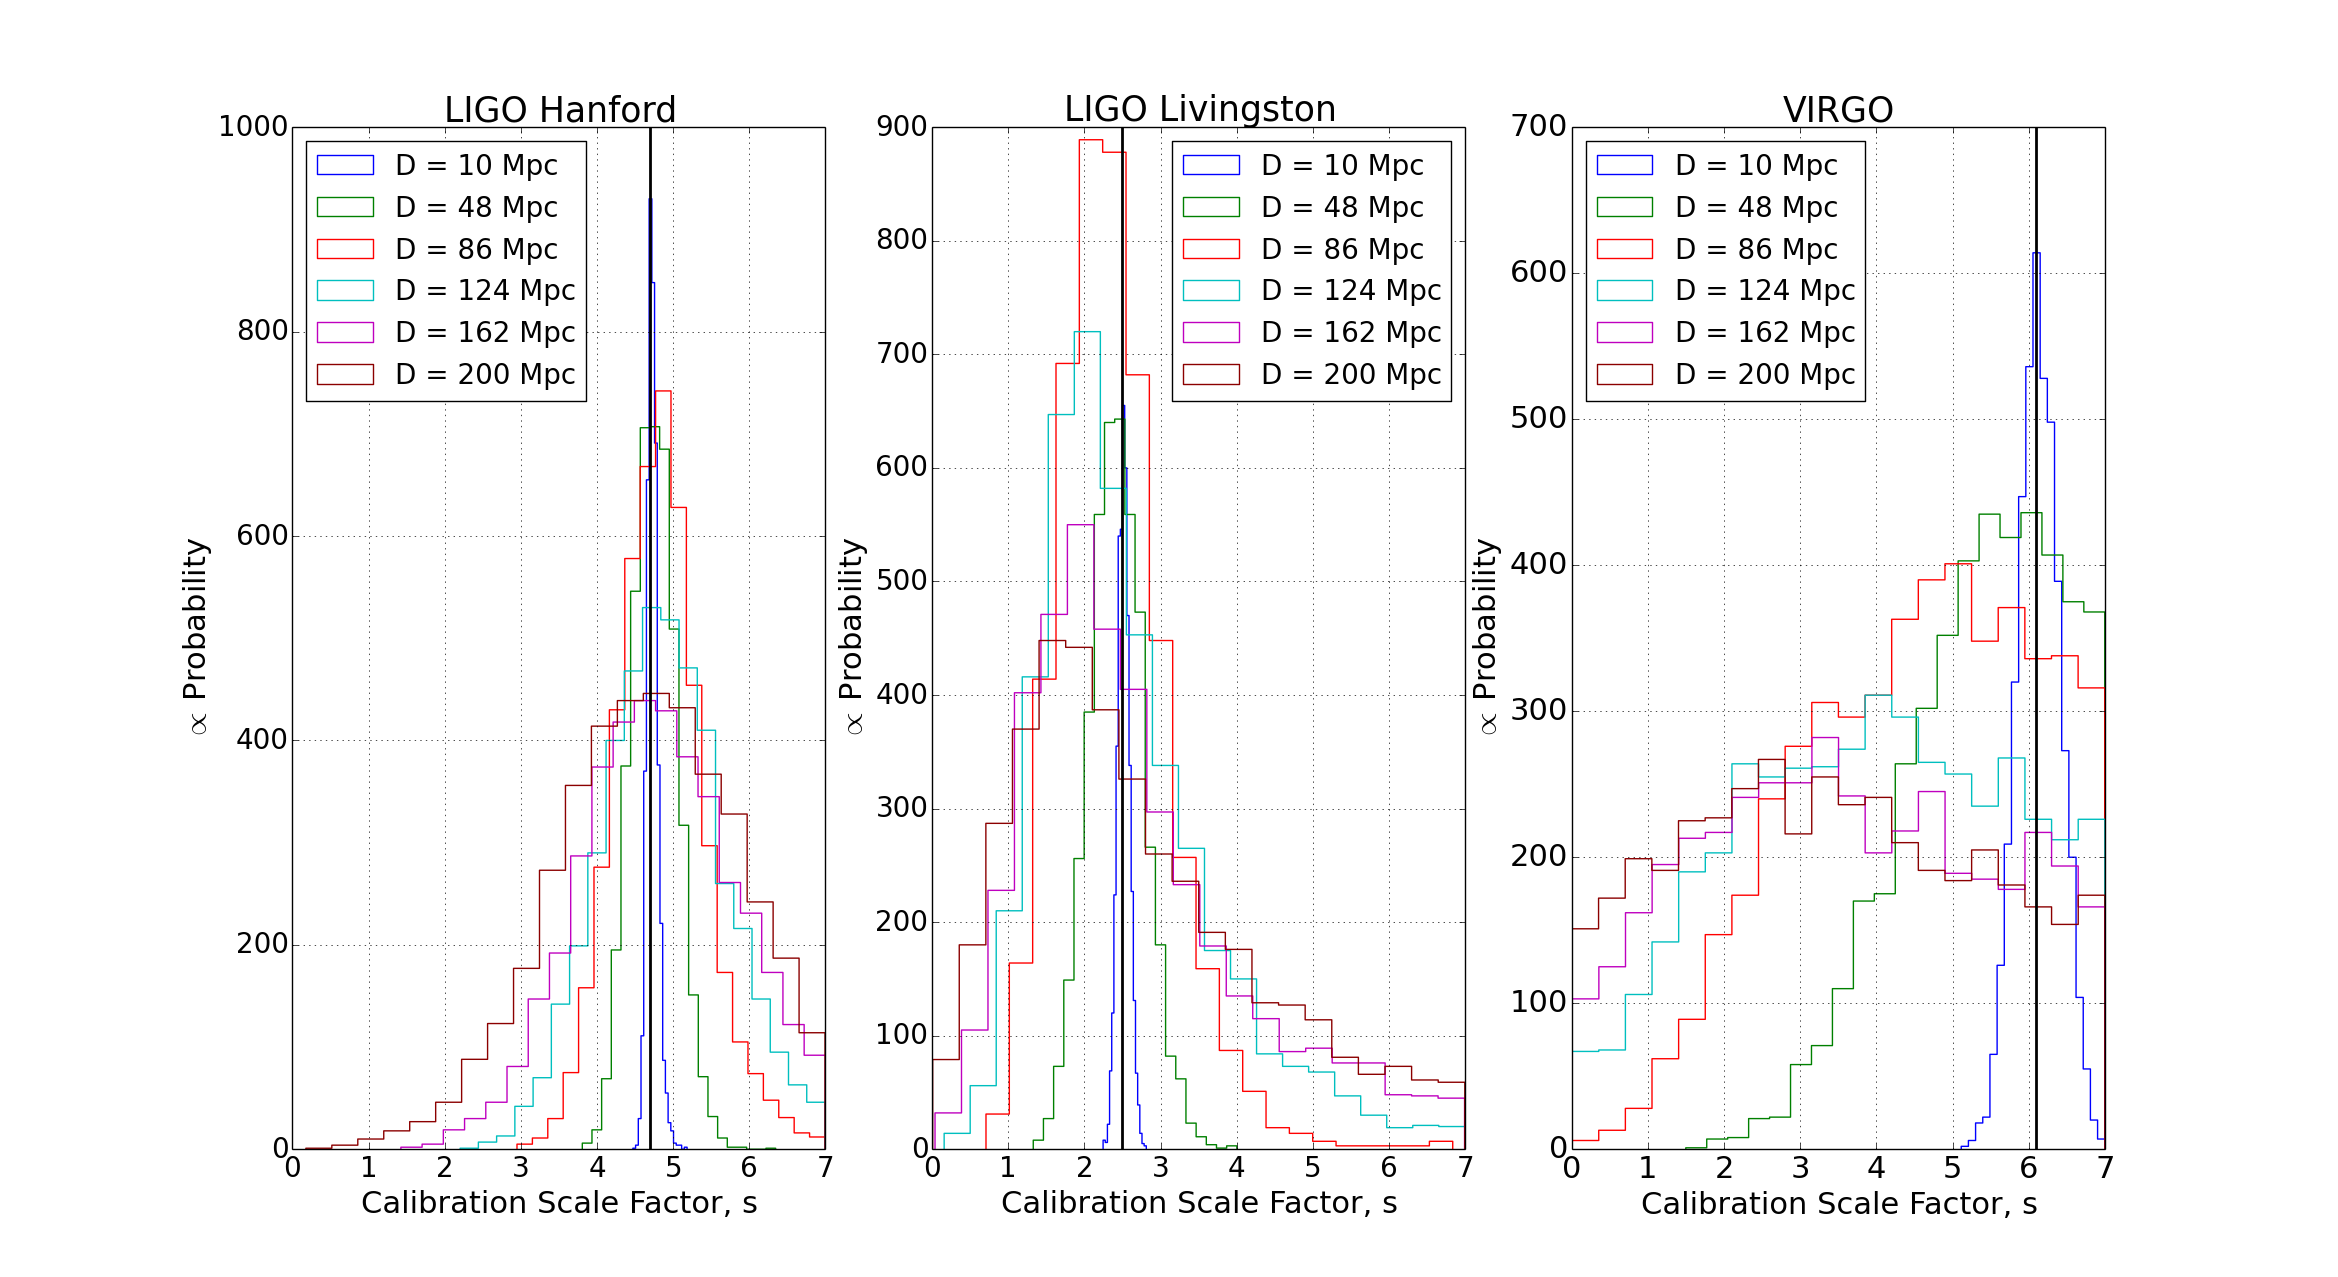
\includegraphics[width = \textwidth]{MD_non_empty_D10_200}
  \caption{Posterior distribution on the calibration scale factor for
all three detectors. Simulations carried out with some prior parameters.}
  \label{fig:mult-non-D}
\end{figure}


The histograms shown in figure~\ref{fig:mult-non-D} were made using the full
range of prior parameters. The uncertainty in the calibration error is larger
with a less known source of GWs. VIRGO, again, has the least certain
calibration error resolution with the distribution becoming even more uniform.
The standard deviation for both LIGO curves become larger with increasing
luminosity distance as before. For $D_{L} = 200Mpc$,  the standard deviation is
$\tilde 30\%$ of the true value. When comparing this to the current method,
this again is not as accurate.

Throughout the duration of this project the antenna patterns were defined by a
randomly chosen sky position, as seen in equation~\ref{eq:gravsig}. This did
not give a true representation of the estimation capable by algorithm as this
position could be a bad one; making parameterisation more difficult and less
precise. To then test this new method of calibration fully, the entire field of
view of the detector must be analysed. The sky positions $\alpha$, $\delta$,
were distributed as: \begin{table}[H] \centering \begin{tabular}{|c|c|} \hline
Parameter & Distribution \\ \hline $\alpha$       & U($0$,$2\pi$) \\
$\sin(\delta)$ & U($-1$,$1$)    \\ \hline \end{tabular} \caption{\textit{The
distribution of sky position. U(a,b) indicates a uniform distribution between a
and b.}} \label{tab:sp} \end{table}

Figures~\ref{fig:snr-rndsp} and~\ref{fig:std-rndsp} were obtained using a
luminosity distance $D_{L} = 200 Mpc$ as this is the expected luminosity
distance predicted to host the first observable GW~\cite{peadvanced}. $100$
different sky positions were tested using the LIGO Hanford site. The number of
locations was limited by the length of time these simulations took to carry
out. Increasing the number of locations would give a more accurate
representation of the estimation ability; this can be carried out in future.
Finally, a full range of prior parameters were also used in the simulation
set-up.

\begin{figure}
  \centering
  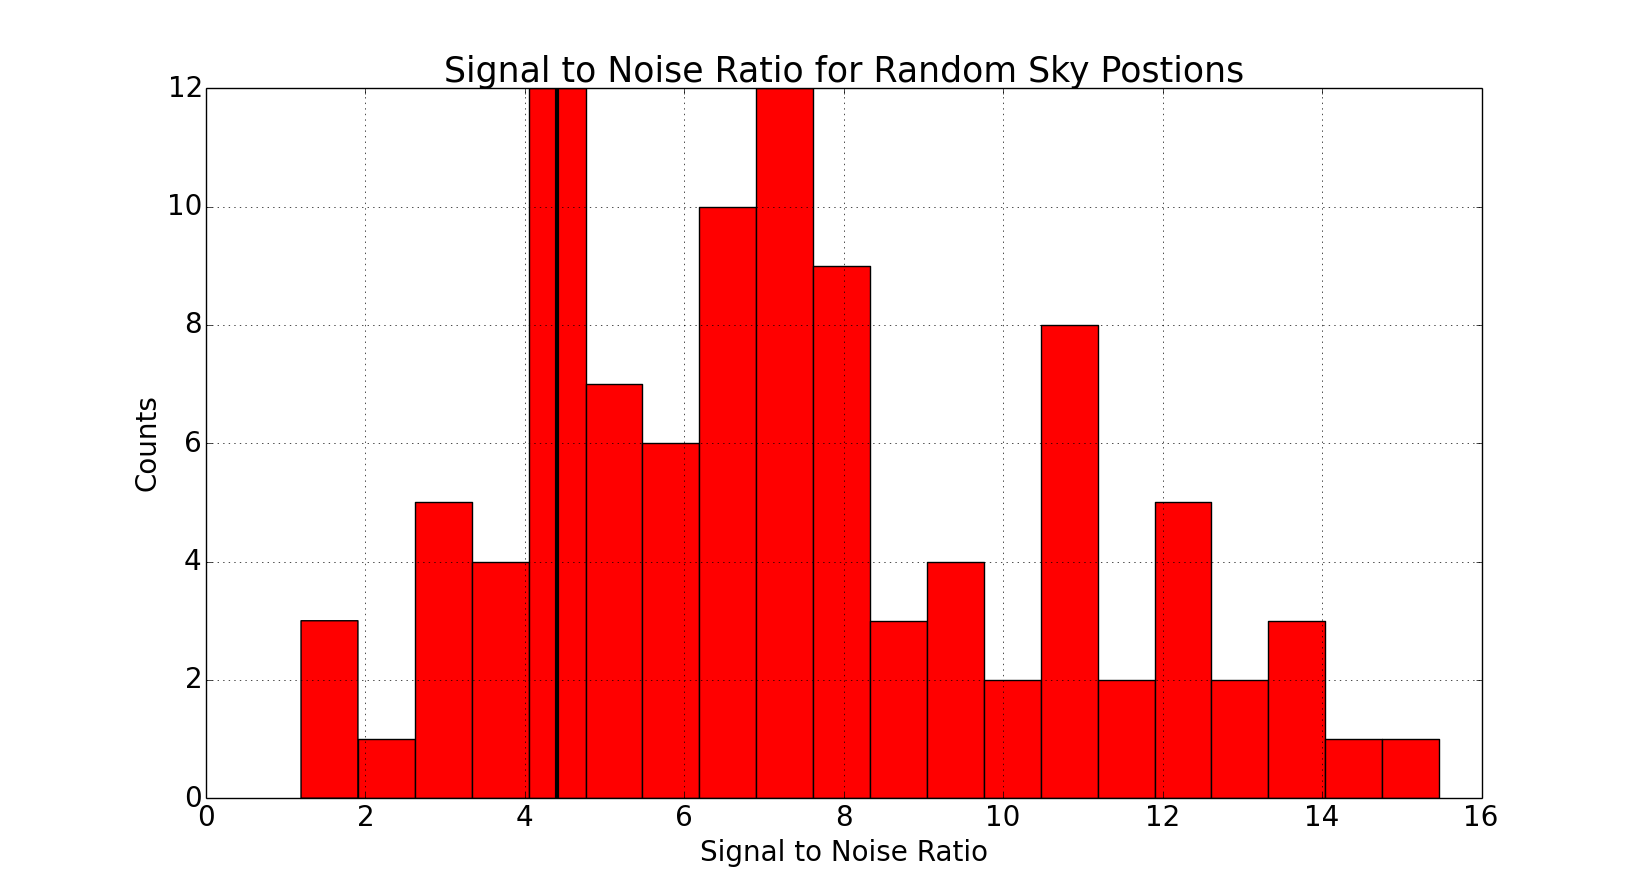
\includegraphics[width=\textwidth]{rand_sp_snr_D200}
  \caption{Signal to noise ratio for every sky position analysed at
$D_{L} = 200 \,Mpc$. The vertical black line represents the SNR for the sky
position used throughout previous simulations}
  \label{fig:snr-rndsp}
\end{figure}

Figure~\ref{fig:snr-rndsp} shows the histogram of SNRs for the entire field of
view for the detector. Predictions state that at a luminosity distance of
$D_{L}=200\,Mpc$, the SNR will be roughly 8. This is consistent with the
results obtained. The vertical black line shown in figure~\ref{fig:snr-rndsp}
represents the SNR used throughout the project using the randomly chosen
$\alpha$ and $\delta$. One can see that this is a less-than-average SNR and may
explain the resolution of the calibration error not being too precise. This
then is a promising result and the full testing of this new calibration method
can be carried out.


\begin{figure}
  \centering
  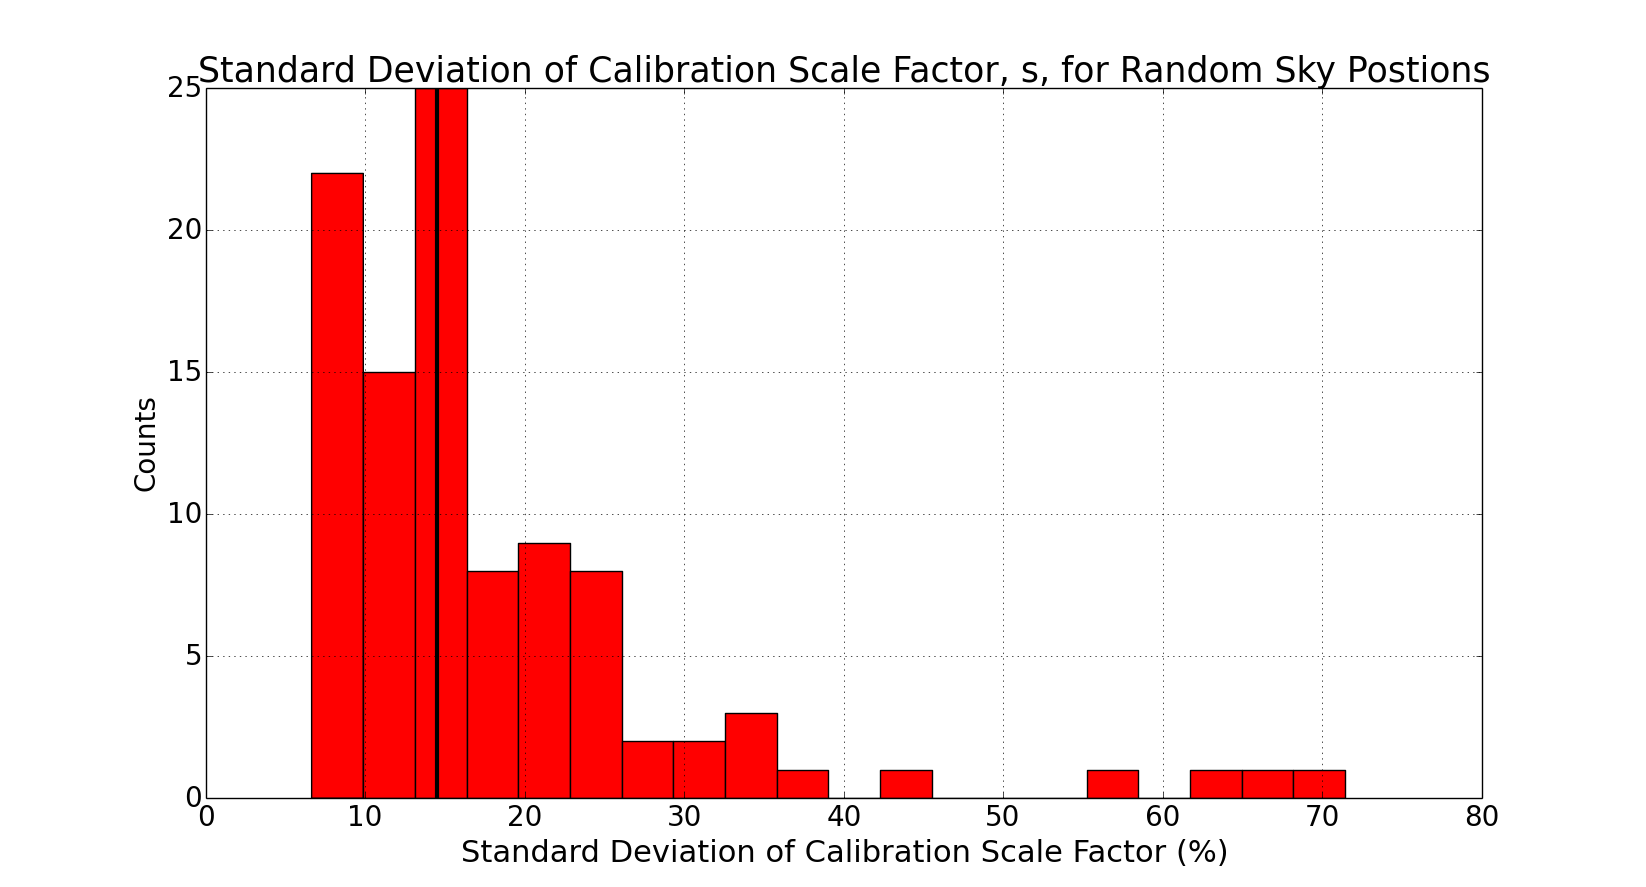
\includegraphics[width=\textwidth]{rand_sp_std_D200}
  \caption{Standard Deviation (as a $\%$ of the true scale factor
value) for every sky position analysed at $D_{L}=\,200Mpc$. The vertical black
line indicates the median of the distribution.}
  \label{fig:std-rndsp}
\end{figure}



Figure~\ref{fig:std-rndsp} is the distribution of fractional standard
deviations on s for each sky position analysed, given as a percentage. The
vertical black line in this figure shows the \textit{median} of the
distribution. The results show that the algorithm can resolve the calibration
error in the data within the range of $\sim 7\%$ to $\sim 14\%$ of the true
value of $s$, for $D_{L}=200\,Mpc$. Being able to recover the scale factor
error to this accuracy range confirms that the new method of calibration method
is very competative with current techniques. These results also confirm that
the sky position used throughout the project was indeed a bad choice with an
error estimation of $\sim 24\%$.


Other simulations relating to the randomisation of $\alpha$ and $\delta$ were
carried out in this project. Different luminosity distances were simulated to
test different levels of SNR. The expected trend was that the standard
deviation scales with SNR; with high SNR yielding a better resolution of the
scale factor error. The results show this trend, given in table

\begin{table}
  \centering
  \begin{tabular}{|c|c|c|}
    \hline
    Distance ($Mpc$) &$\langle$ SNR $\rangle$ & median(Standard
Deviation)($\%$) \\
    \hline
    $20$ & 74 & 1.5 \\
    $120$ & 12  & 7 \\
    $450$ & 3 & 27\\
    \hline
  \end{tabular}
  \caption{\textit{Random sky positions for different luminosity distances;
$\langle$SNR$\rangle$ is the mean SNR for the distribution. }}
  \label{tab:dist-randsp}
\end{table}

The last, and lengthiest, set of simulations carried out used a network of
detectors. Analysis on a luminosity distance of $200 \,Mpc$ was the only one
carried out in this paper. This was due to time taken to process these
simulations. With a full prior range and $100$ random sky positions as before,
the standard deviations and SNRs were obtained. Results are shown
in~\ref{tab:mult-rndsp}.


\begin{table}
\centering
\begin{tabular}[H]{|c|c|c|}
\hline
  Detector   & $\langle$SNR$\rangle$ & median(Standard Deviation)($\%$)\\
\hline
LIGO Hanford & 20& 3 \\
LIGO Livingston & 20 & 10 \\
Virgo & 5 & 30\\
\hline
\end{tabular}
\caption{\textit{Results from randomising the sky position using a network of
detectors with a full range of prior parameters at $D_{L} = 200\, Mpc$.}}
\label{tab:mult-rndsp}
\end{table}


Table~\ref{tab:mult-rndsp} gives promising results for both LIGO sites. One can
see that the error estimation for LIGO Hanford is very good, with half of the
positions analysed having an uncertainty $<3\%$. One would expect the gap in
estimation accuracy between the two LIGO sites to be smaller as they are built
to the same sensitivity. This leads to the conclusion that not enough sky
positions were analysed. Virgo again has a less accurate recovery of the
calibration scale factor. As mentioned above, the larger uncertainty is
expected to originate from the sensitivity of the detector itself.

%%%%%%%%%%%%%%%%%%%%%%%%%%%%%%%%%%%%%%%%%%%%%%%%%%
%%%%%%%%%%%%%%%%%%%%%%%%%%%%%%%%%%%%%%%%%%%%%%%%%%
\section{Distance estimates from \acp{sGRB}\label{sec:cosmo}}

~\cm{Describe the cosmological analysis used to obtain the distance from the
GRB}

%%%%%%%%%%%%%%%%%%%%%%%%%%%%%%%%%%%%%%%%%%%%%%%%%%
%%%%%%%%%%%%%%%%%%%%%%%%%%%%%%%%%%%%%%%%%%%%%%%%%%
\section{Multiple events without counterpart\label{sec:multiple}}

\cm{A discussion of the issues regarding multiple events
without EM counterparts.}

%%%%%%%%%%%%%%%%%%%%%%%%%%%%%%%%%%%%%%%%%%%%%%%%%%
%%%%%%%%%%%%%%%%%%%%%%%%%%%%%%%%%%%%%%%%%%%%%%%%%%
\section{Discussion\label{sec:discussion}}

\cm{What did we learn.}

This paper has shown that for differing levels of SNR, the error in the
calibration is resolved within a certain accuracy range. Initial simulations
used a bad sky position, resulting a low SNR which created larger uncertainty
in resolving $s$. It was shown that for this sky position, the calibration
scale factor estimation was recovered with an accuracy of roughly a $27\%$ for
$D_{L} = 200\,Mpc$ for LIGO Hanford. The resolution of $s$ for a network of
detectors was also shown.

The main results obtained in this project were from analysing randomly chosen
sky positions from the entire field of view for the detector. Through these
simulations, it was shown that this new method of calibration can reach and
surpass the current method in terms of accuracy. The results in
figure~\ref{fig:std-rndsp} show that for half of the randomly chosen sky
positions relate to an estimation of $s$ within a range comparable with the
current methods.

These results are reassuring for parameter estimation of the defining GW signal
and would help in reducing the uncertainty in a direct detection. This project
was; however, time constrained. There are many, many things that could be done
with this project. A true noise realisation with each frequency bin having a
random Gaussian noise would be the next step in calibration error estimation.

This project is only the beginning in testing this new method of calibration.
More rigorous testing has to be carried out for a number of different systems.
As mentioned above, a larger number of random sky positions have to be analysed
to give better understanding of the resolution capabilities of the method. The
current technique of calibration defines the error in the detector to be a
complex function of frequency and phase of the GW. Instead of the simple scale
factor used so far, a more realistic error can be tested to ensure that the
estimation in its value is still comparable with current methods.


For applications of this calibration method, hypothesis testing could be
carried out. Testing different hypothesis is the technique used in determining
a GW signal in a data-set when compared to a noise-only data-set. Being able to
show with confidence that the data contains a signal is the primary focus of GW
research at the moment. Therefore if uncertainty can be removed from the
analysis this will ensure a more confident detection. Using this new method is
resolving and removing the uncertainty is an area which has to be explored.

\MP{We emphasise that our work has assumed that the PSD used in the likelihood function
for estimating the calibration scale factor is an accurate representation of the
PSD at the time of the observed CBC signal. In reality the PSD may be estimated from
a period close to, but not overlapping, the signal time and therefore may be slightly
different (see e.g. \cite{2013PhRvD..88h4044L}). Our result would therefore be completely correlated
with any uncertainty in the PSD estimate, but would still offer an upper limit
on the calibration uncertainty.}

\MP{The BayesLine algorithm \cite{2015PhRvD..91h4034L} may provide a natural
way to perform this analysis in particular when accounting for a frequency
dependent calibration.}

\ack

We would like to acknowledge the useful discussions with a whole bunch
of people.

\section*{References}

\bibliographystyle{unsrt}
\bibliography{masterbib}
\end{document}


